\documentclass{beamer}

\usetheme{CambridgeUS}
%\usetheme{Luebeck}
\usecolortheme{beaver}
\useinnertheme{rectangles}
\usepackage[utf8]{inputenc}
\usepackage[czech]{babel}
\usepackage{graphicx}
\usepackage{amsmath}
\usepackage{color}
\usepackage{listings}
\lstset{
    breaklines=true,
    xleftmargin=\parindent,
    language=C++,
    showstringspaces=false,
    basicstyle=\footnotesize\ttfamily,
    keywordstyle=\color[rgb]{0,0,1},
    commentstyle=\color[rgb]{0.026,0.112,0.095},
    %identifierstyle=\color{blue},
    stringstyle=\color[rgb]{0.627,0.126,0.941},
}

\begin{document}
\setbeamertemplate{caption}{\raggedright\insertcaption\par}

\title[ReCodEx -- ReCodEx Code Examiner] % (optional, only for long titles)
{ReCodEx -- ReCodEx Code Examiner}
\author[Buchar, Polanka, Rozsíval, Stefan]{J. Buchar, M. Polanka, Š. Rozsíval, P. Stefan}
\institute[] % (optional)
{
  Matematicko-fyzikální fakulta\\
  Univerzita Karlova v Praze
}
\date[3. 12. 2016]{} % (optional)
\subject{Computer Science}
%\logo{
\includegraphics[width=0.2\textwidth]{images/logo_recodex.png}}
\titlegraphic{
\includegraphics[width=0.5\textwidth]{images/logo_recodex.png}}

\frame{\titlepage}

\section{ReCodEx}

\begin{frame}
	\frametitle{Motivace}
	\begin{itemize}
		\item Zastaralý frontend CodExu
		\item Sandbox nepodporuje paralelní programy
		\item Omezená vyhodnocovací pipeline (kompilace/spuštění/vyhodnocení)
		\item Pevně svázané komponenty CodExu
		\item Nutnost separátních instancí pro různé programovací jazyky
	\end{itemize}
\end{frame}

\begin{frame}
	\frametitle{Praktická ukázka}
\end{frame}

\begin{frame}
	\frametitle{Architektura}
	\begin{itemize}
		\item Nezávislé komponenty, které spolu komunikují po síti
		\item Webová aplikace je výchozí uživatelské rozhraní pro REST API
		\item REST API 
			\begin{itemize}
				\item uchovává a poskytuje data
				\item zprostředkovává vyhodnocení úloh
			\end{itemize}
		\item Backend zajišťuje bezpečné vyhodnocování úloh
	\end{itemize}
\end{frame}

\begin{frame}
	\frametitle{Komponenty a komunikace}
	\begin{center}
		\includegraphics[width=0.8\textwidth]{images/communication.png}
	\end{center}
\end{frame}

\begin{frame}
	\frametitle{Webová aplikace}
	\begin{center}
		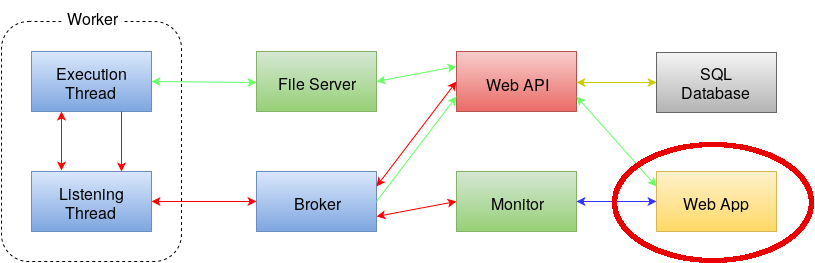
\includegraphics[width=0.6\textwidth]{images/communication-webapp.png}
	\end{center}
	\begin{itemize}
		\item ovládání systému uživateli
		\item SPA (single-page application)
		\item ECMAScript a HTML5
		\item založena na React/Redux
		\item NodeJS server -- lepší výkon kvůli předrenderování na serveru
	\end{itemize}
\end{frame}

\begin{frame}
	\frametitle{REST API}
	\begin{center}
		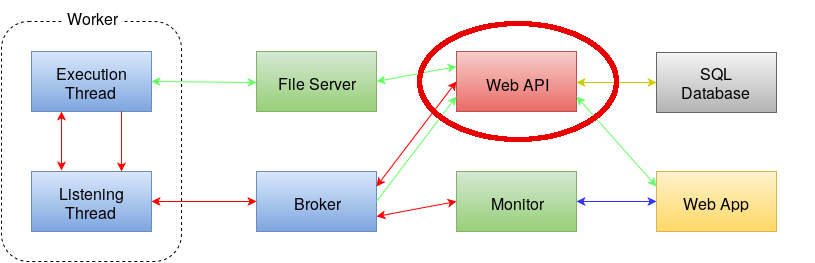
\includegraphics[width=0.6\textwidth]{images/communication-webapi.png}
	\end{center}
	\begin{itemize}
		\item hlavní logika aplikace, ukládání dat, komunikace s backendem
		\item PHP 7
		\item Nette web framework, Doctrine ORM, ZeroMQ messaging, \dots
		\item Apache server s {\it mod\_php}
		\item MySQL databáze (MariaDB)
		\item Autentizace -- lokální, CAS
	\end{itemize}
\end{frame}

\begin{frame}
	\frametitle{Broker}
	\begin{center}
		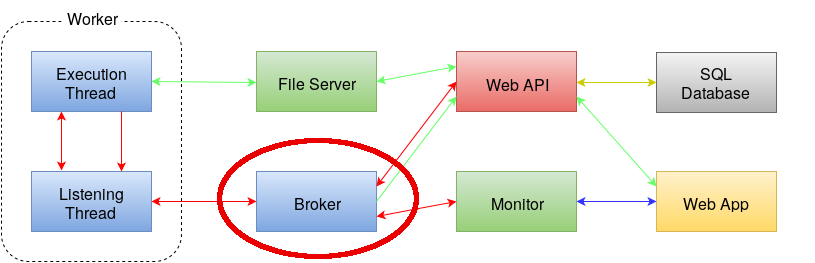
\includegraphics[width=0.6\textwidth]{images/communication-broker.png}
	\end{center}
	\begin{itemize}
		\item rozdělování práce mezi více workerů
			\begin{itemize}
				\item workeři se mohou lišit (hardware, běhová prostředí, \dots) 
					-- rozdělování úloh podle kritérií, load balancing
				\item fault tolerance -- přerozdělování úloh při pádu workera
			\end{itemize}
		\item C++11
		\item ZeroMQ, libcurl, \dots
		\item \texttt{systemd} služba
	\end{itemize}
\end{frame}

\begin{frame}
	\frametitle{Worker}
	\begin{center}
		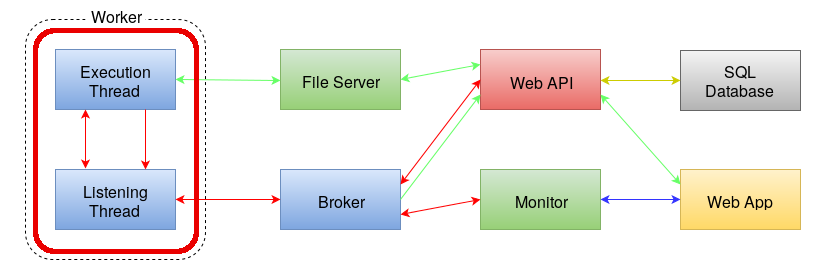
\includegraphics[width=0.6\textwidth]{images/communication-worker.png}
	\end{center}
	\begin{itemize}
		\item bezpečné zpracování a vyhodnocení úlohy (sandbox isolate)
			\begin{itemize}
				\item založeno na Linux kernel namespaces a CGroups
				\item umožňuje rozumně přesné měření času a paměti
			\end{itemize}
		\item podpora Windows je možná (existuje prototyp)
		\item C++11
		\item ZeroMQ, libcurl, libarchive, \dots
		\item \texttt{systemd} služba
	\end{itemize}
\end{frame}

\begin{frame}
	\frametitle{Konfigurace úlohy}
	\begin{itemize}
		\item velmi přizpůsobitelná různým druhům použití
		\item strukturovaná textová reprezentace (YAML)
		\item jednoduché tasky (fetch url, decompress, \dots) spojené závislostmi
		\item \textit{interní} a \textit{externí} tasky
	\end{itemize}
\end{frame}

\begin{frame}
	\frametitle{Fileserver}
	\begin{center}
		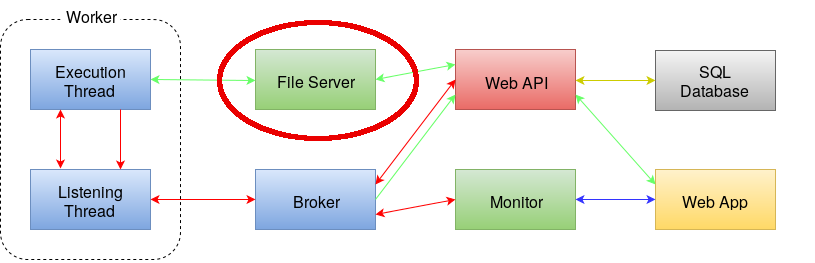
\includegraphics[width=0.6\textwidth]{images/communication-fileserver.png}
	\end{center}
	\begin{itemize}
		\item ukládání studentských řešení a výsledků vyhodnocení
		\item skladování pomocných souborů k úlohám
			\begin{itemize}
				\item hash obsahu jako jméno souboru $\rightarrow$ částečné odstranění duplicit
			\end{itemize}
		\item oddělení od REST API $\rightarrow$ více instancí API může sdílet úložiště (load~balancing, \dots)
		\item Python 3 a webový framework Flask
		\item WSGI aplikace nasazená na Apache s {\it mod\_proxy} a uWSGI
	\end{itemize}
\end{frame}

\begin{frame}
	\frametitle{Monitor}
	\begin{center}
		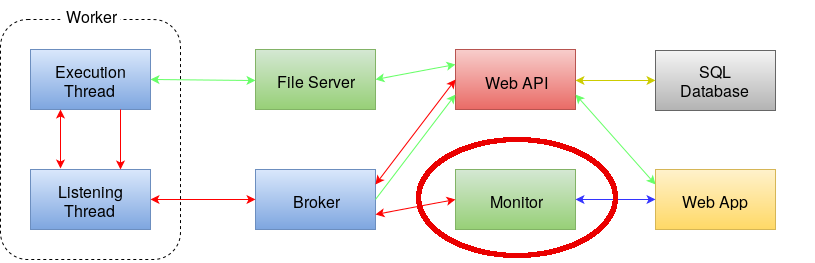
\includegraphics[width=0.6\textwidth]{images/communication-monitor.png}
	\end{center}
	\begin{itemize}
		\item hlášení postupu vyhodnocení webové aplikaci
		\item umožňuje zobrazení výsledků bez aktivního čekání
		\item Python 3
		\item ZeroMQ nadstavba pro Python, websockets, asyncio, \dots
		\item \texttt{systemd} proces
	\end{itemize}
\end{frame}

\begin{frame}
	\frametitle{Scénář -- vyhodnocení úlohy}
	\begin{center}
		\includegraphics[width=0.8\textwidth]{images/communication.png}
	\end{center}
\end{frame}

\begin{frame}
	\frametitle{Shrnutí}
	\begin{itemize}
		\item návrh a implementace nového vyhodnocovacího systému
		\item zapracování požadavků MFF UK
		\item moderní technologie, rozšiřitelnost, bezpečnost
		\item automatizované testování
		\item plné nasazení v příštím akademickém roce
	\end{itemize}
\end{frame}

\begin{frame}
	\frametitle{Náměty k vylepšení}
	\begin{itemize}
		\item ovládací prvky ve webové aplikaci na základě zpětné vazby uživatelů
		\item formuláře pro přidání a zadávání úloh
		\item přehlednější hlášení chybových stavů
	\end{itemize}
\end{frame}

\section{Závěr}
\begin{frame}
	\frametitle{Závěr}
	\centering
	\LARGE{Děkujeme za pozornost}
\end{frame}

\end{document}
